A limit cycle is an \emph{isolated closed trajectory}.
\emph{Isolated} means that neighboring trajectories are not closed; they spiral either toward or away from the limit cycle.
\begin{figure}[H]
	\centering
	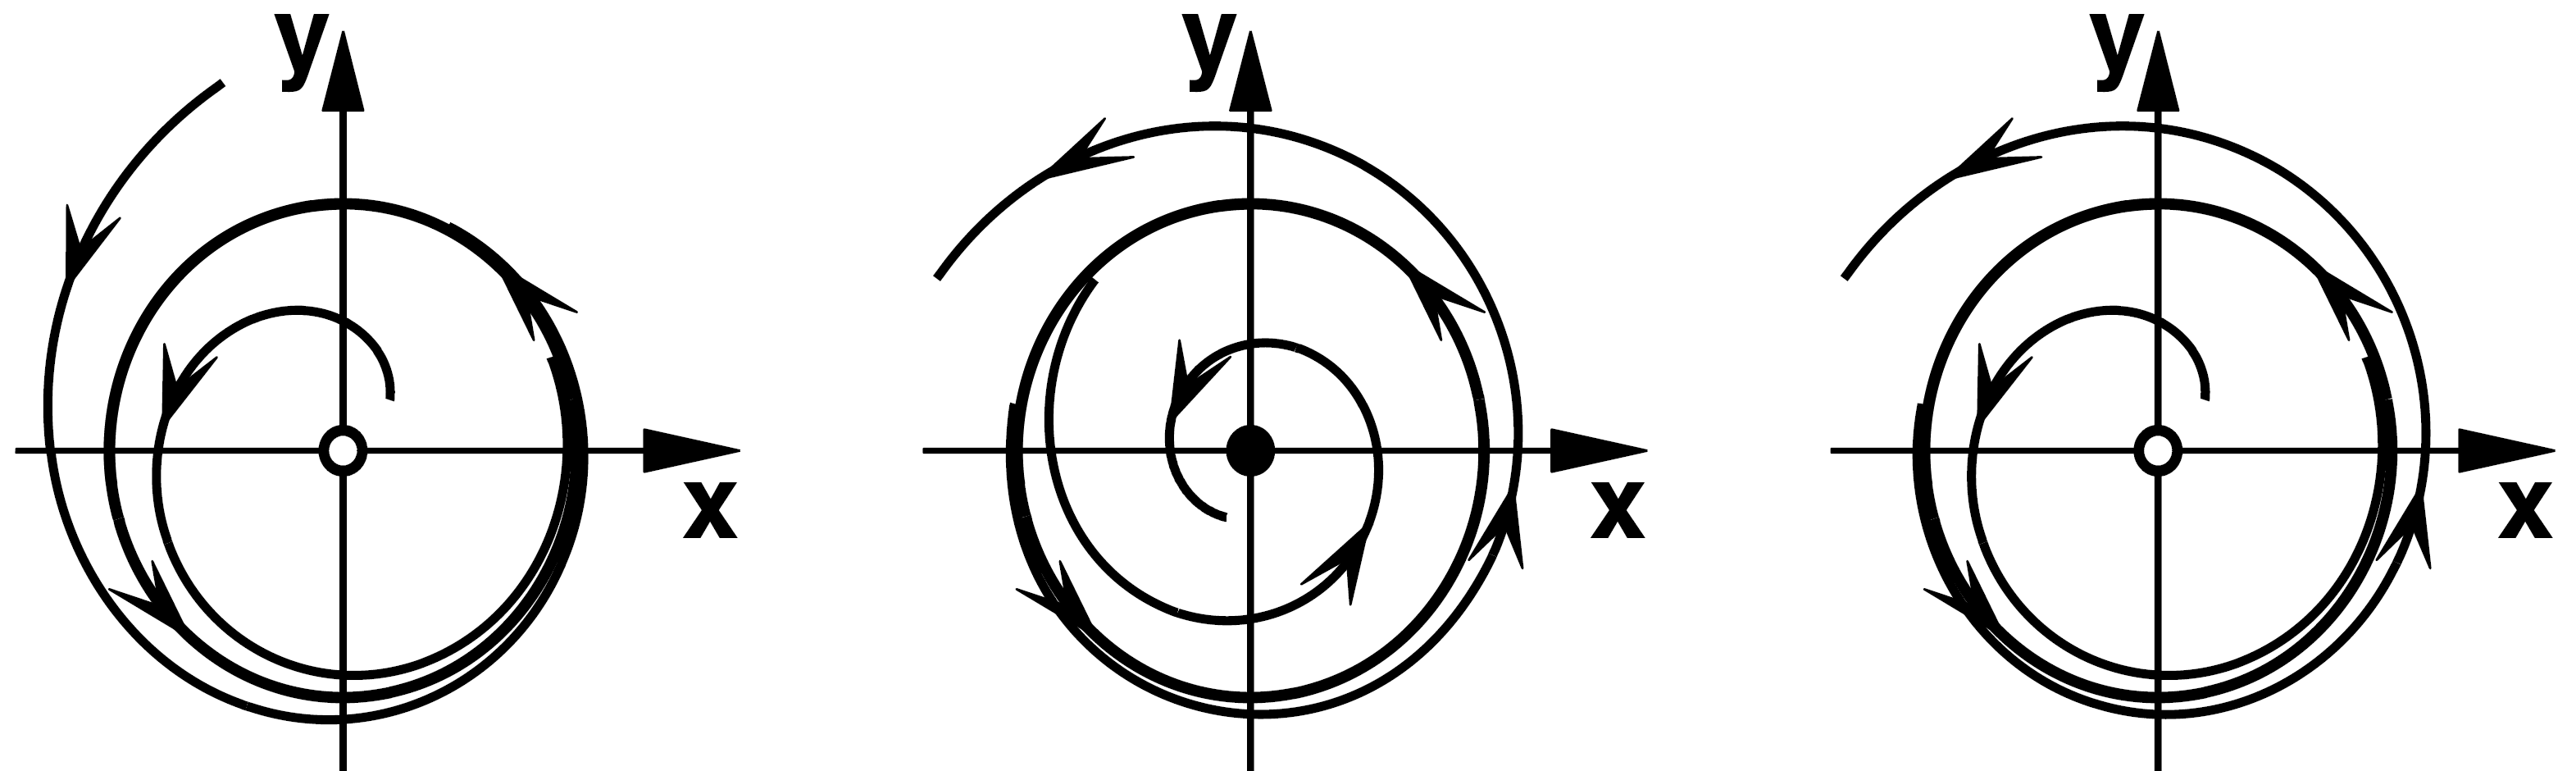
\includegraphics[width=0.5\linewidth]{tlc.png}
	\caption{Limit cycles attracting or/and repelling neighboring trajectories. Stable (right), unstable (middle), half-stable (right)}
	\label{fig:tlc}
\end{figure}
A \emph{stable} limit cycle attracts trajectories from its outside and its inside, whereas an \emph{unstable} limit cycle repels trajectories on both sides.
A \emph{half-stable} limit cycle attract the trajectories from one side and repel those on the other.\\
It is intuitively clear that inside a stable limit cycle there must be an unstable fixed point and vic-versa (Figure (\ref{fig:tlc})).
\subsection{Closed Orbits}
\begin{theorem}[\textbf{Gradient System}]
	\emph{Closed orbits and Limit Cycles are impossible} if the systems can be written in the form $\mathbf{\dot{x}}=-\nabla V$ for some continuously differentiable, single-valued scalar function $V(x)$. 
\end{theorem}
\begin{proof}
	Suppose there were a closed orbit. We obtain a contradiction by considering the change in $V$ after one circuit.
	On the one hand, $\Delta V=0$ since $V$ is single-valued.
	But on the other hand,
	\begin{equation}
		\Delta V=\int_0^T\frac{dV}{dt}\mathop{dt}=\int_0^T(\Delta V\cdot\mathbf{\dot{x}})\mathop{dt}=-\int_0^T\|\mathbf{\dot{x}}\|^2\mathop{dt}<0 
	\end{equation}
	If $\mathbf{\dot{x}}=0$ the trajectory is a fixed point, not a closed orbit.
	This contradiction shows that closed orbits can’t exist in gradient systems. 
\end{proof}
\begin{theorem}[\textbf{Lyapunov Function}]
	Consider Case 2. of Theorem (\ref{thm:lst}).\\
	Here $\mathbf{\tilde{x}}$ is globally asymptotically stable: for all initial conditions, $\mathbf{x}(t)\rightarrow\mathbf{\tilde{x}}$ as $t\rightarrow\infty$.\\
	In particular the system has \emph{no closed orbits}.
\end{theorem}
\begin{theorem}[\textbf{Bendixson’s Negative Criterion}]
	There are \emph{no closed paths} in a simply connected region of the phase plane of the system on which $\left(\dfrac{\partial f_1}{\partial x_1}+\dfrac{\partial f_2}{\partial x_2}\right)$ is not identically zero and is of one sign.
\end{theorem}
\begin{theorem}[\textbf{Dulac’s Criterion}]
	Let $\mathbf{\dot{x}}=\mathbf{f(x)}$ be a continuously differentiable vector field defined on a simply connected subset $R$ of the plane.
	If there exists a continuously differentiable, real-valued function $g(\mathbf{x})$ such that $\nabla\cdot(g\mathbf{\dot{x}})$ has one sign throughout $R$, then there are \emph{no closed orbits} lying entirely in $R$.
\end{theorem}
\begin{proof}
	Suppose there were a closed orbit $C$ lying entirely in the region $R$. Let $A$ denote the region inside $C$. Then Green’s theorem yields
	\begin{equation}
		\iint_A\nabla\cdot(g\mathbf{\dot{x}})\mathop{dA}=\oint_Cg\mathbf{\dot{x}}\cdot\mathbf{n}\mathop{d\ell}
	\end{equation}
	Where $\mathbf{n}$ is the outward normal and $d\ell$ is the element of arc length along $C$.
	Look first at the double integral on the left: it must be \emph{nonzero}, since $\nabla\cdot(g\mathbf{\dot{x}})$ has one sign in $R$.
	On the other hand, the line integral on the right equals \emph{zero} since $\mathbf{\dot{x}}\cdot\mathbf{n}=0$ everywhere, by the assumption that $C$ is a trajectory (the tangent vector $\mathbf{\dot{x}}$ is orthogonal to $\mathbf{n}$).
	This contradiction implies that no such $C$ can exist.
\end{proof}
The following theorem gives the criterion for a system to have finite number of limit cycles.
\begin{theorem}[\textbf{Dulac}]
	In any bounded region of the plane, a planar analytic system $\dot{x}=f(x)$ analytic in $\mathbb{R}^2$ has at most a finite number of limit cycles.
	In other words, any polynomial system has at most a finite number of limit cycles in $\mathbb{R}^2$.
\end{theorem}
\begin{theorem}[\textbf{Poincar\'e}]
	A planar analytic system (\ref{eq:2d}) cannot have an infinite number of limit cycles that accumulate on a cycle of (\ref{eq:2d}).
\end{theorem}
\subsection{Poincar\'e--Bendixson Theorem}
This theorem helps in finding methods to establish that closed orbits exist in particular systems.
\begin{wrapfigure}{r}{0.3\textwidth}
	\centering
	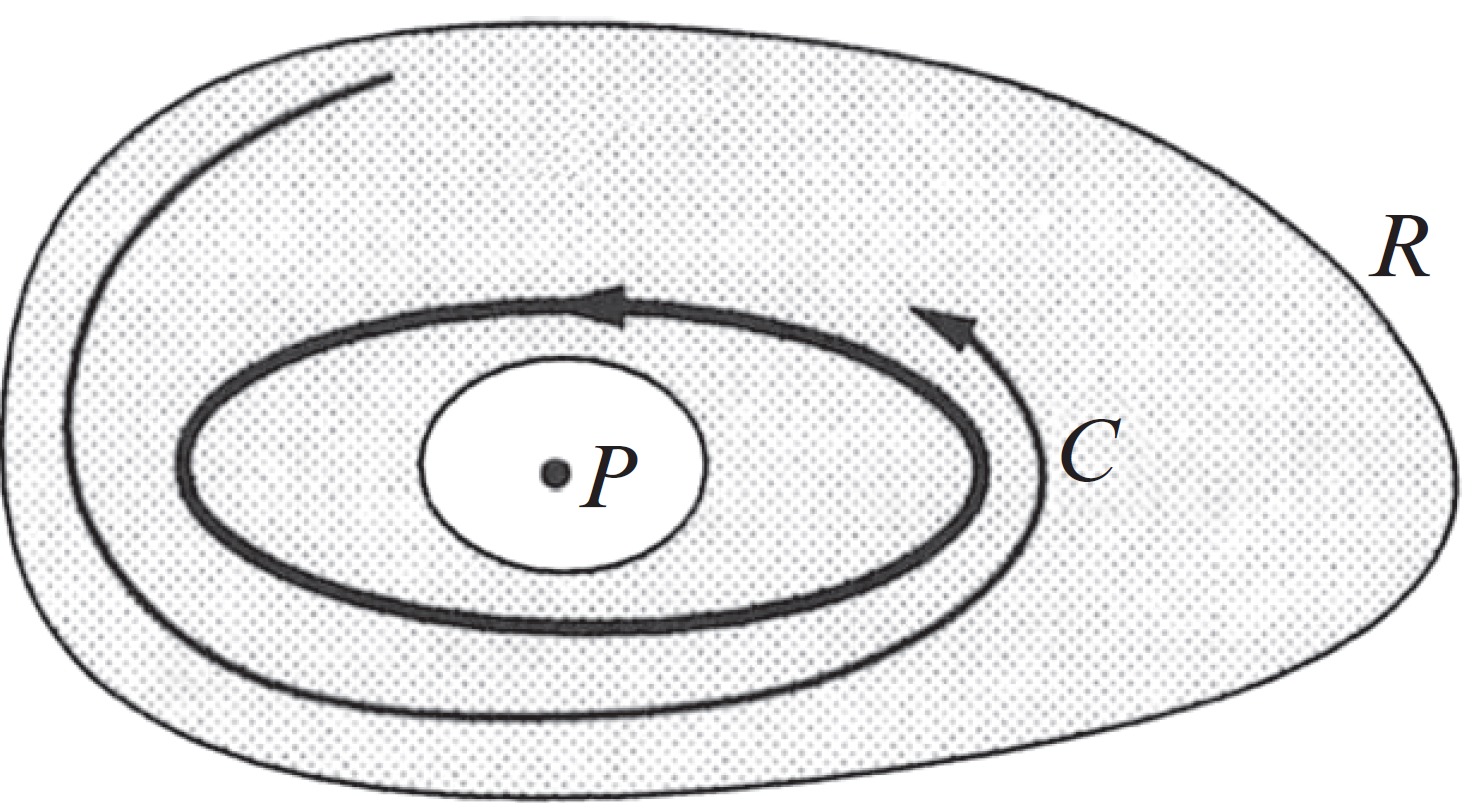
\includegraphics[width=0.25\textwidth]{pbt.png}
	\caption{}
	\label{fig:pbt}
\end{wrapfigure}
\begin{theorem}[\textbf{Poincar\'e--Bendixson Theorem}]
	Suppose that:
	\begin{itemize}
		\item $R$ is a closed, bounded subset of the plane.
		\item $\mathbf{\dot{x}=f(x)}$ is a continuously differentiable vector field on an open set containing $R$.
		\item $R$ does not contain any fixed points.
		\item There exists a trajectory $C$ that is \emph{confined}in $R$, in the sense that it starts in $R$ and stays in $R$ for all future time (Figure (\ref{fig:pbt})).
	\end{itemize}
	Then either $C$ is a closed orbit, or it spirals toward a closed orbit as $t\rightarrow\infty$.
	In either case, \emph{$R$ contains a closed orbit} (shown as a heavy curve in Figure (\ref{fig:pbt})). 
\end{theorem}